% \SetPicSubDir{ch-Rice}
% \SetExpSubDir{ch-Rice}

\chapter{Literature Review}
\label{ch:literature}
In this chapter, we lay out the foundation of blockchains and explore a systematic exposition on their recent progress.
We organize the review based on the abstract layers as classified in Figure~\ref{diagram:intro:arch}, before identifying the research gap. 

\section{Data Model Layer}
\label{literature:sec:datamodel}
The data model in blochchains concerns on how to organize data that reflect the latest states, and model the ledger that record the historical transactions. 

\subsection{State Organization}
There are two state organizations in the blockchains, the unspent transaction output-based (UTXO) and the account-based. Their key difference lies whether systems explicitly maintain the states. we illustrate both schemes in Figure~\ref{diagram:literature:data_model}.

\begin{figure}
    \centering
    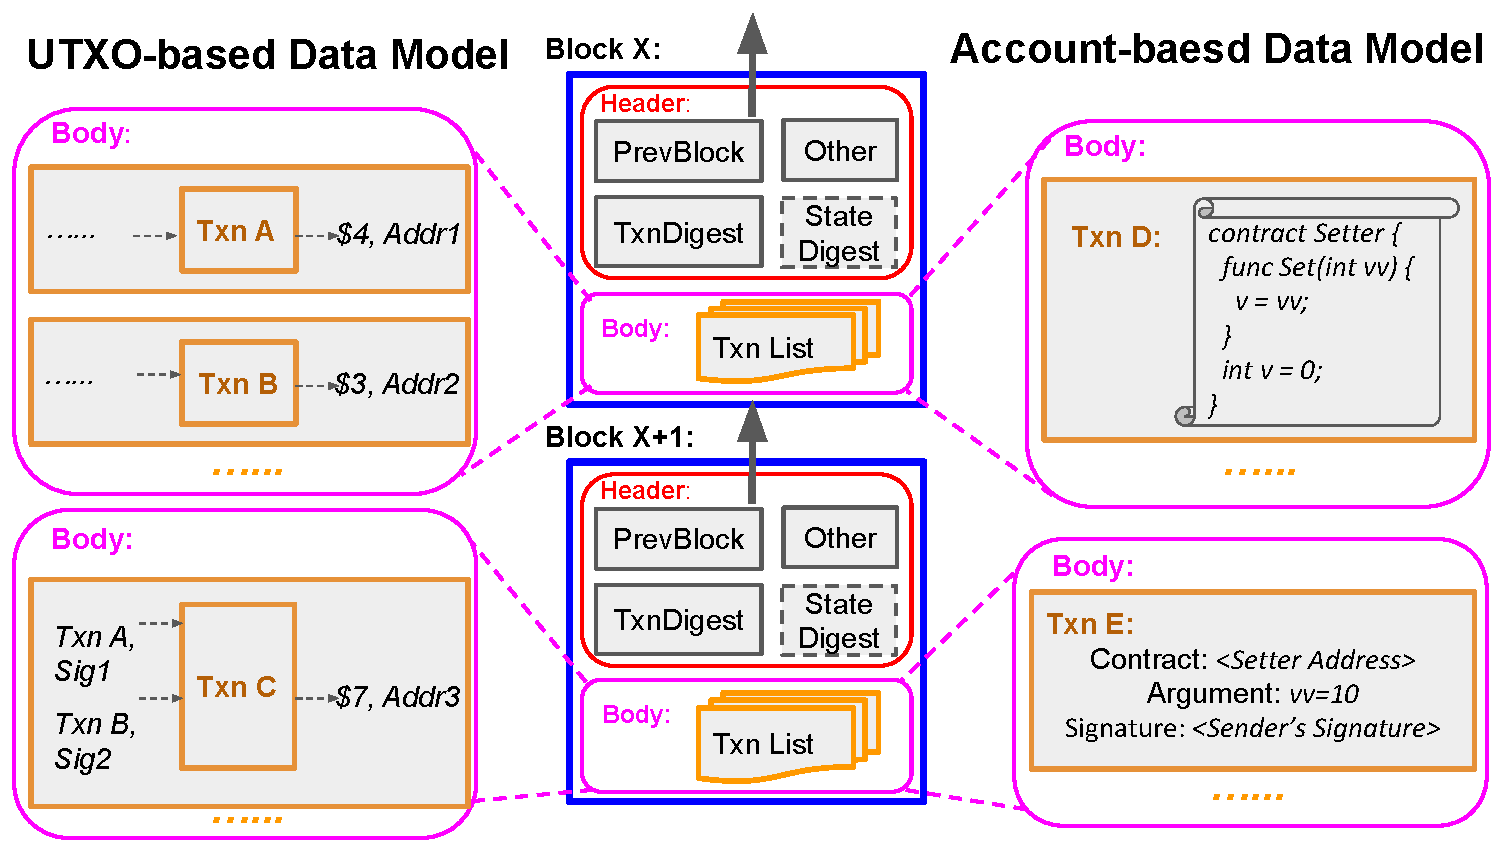
\includegraphics[width=0.8\linewidth]{diagram/literature/data_model.pdf}
    \vspace{\BeforeCaptionVSpace}
    \caption{Unspent Transaction Output (UTXO) model vs the Account-based model. }
    \label{diagram:literature:data_model}
\end{figure}

\textbf{UTXO Model.}
UTXO purely operates on the transaction basis. In their structure, a transaction consists of multiple inputs and outputs. Each output is associated with an amount of cryptocurrency and an unanswered cryptographic puzzle. Any future transaction can reclaim this amount in its input, by providing the puzzle answer and referencing the previously unspent output. An canonical puzzle and its solution can be an address in the format of a public key hash, and a digital signature from the corresponding private key. Notably, the UTXO model does not bookkeep the balance to addresses. All transactions in the ledger form a Direct Acyclic Graph that records the cryptocurrency flow, where identity hides under the anonymous addresses. 

Bitcoins, due to its decentralization and anonymity, provide a terrain for financial crimes, such as drug dealing and the money laundry. There are a number of attempts to exploit the transactional graph, and identify the pattern for the detection~\cite{fleder2015bitcoin,ron2013quantitative,weber2019anti}. 
Some analysis relies on the graph linkage to discover the identity~\cite{ober2013structure,gaihre2018bitcoin,moser2013anonymity} or other information to predict the bitcoin price~\cite{greaves2015using}. 

\textbf{Account-based Model.}
Despite its simplicity, the UTXO model is solely applicable to cryptocurrency-based platforms. 
To support more general workloads, Ethereum introduces the smart contract to encode Turing-complete logic. 
In their design, a transaction either takes in the form of a contract deployment with the executable code. 
Or a transaction provides the execution context to invoke a contract. 
In all cases, each transaction is tagged with the digital signature of the sender. 
In addition, each blockchain peer must explicitly compute for contract states, including the cryptocurrency balance, in each account. 
Such requirement is enforced by the blockchain protocol that all peers shall reach consensus on a post-execution state digest in the block header. 
In contrast, the UTXO-based blockchain only requires for a digest on the transaction integrity.

The account-based data model with smart contracts transition a blockchain into a more general processing platform. 
But it inevitably incurs more vulnerability from the additional complexity. 
For example, some malicious users might run an infinite loop in a transaction to waste system resources. 
To defer such Denial-of-service Attack in the permissionless setting, all blockchains are designed with an incentive-compatible mechanism to prevent the abusive usage. 
For example, Ethereum charges transaction senders with the transaction fee, in a n amount proportional to the number and the complexity of contract operations~\cite{wood2014ethereum}.
Despite this, computational-heavy transactions may still render blockchains securely-flawed: some researchers reveal that rational block validators tend to skip their execution to gain an edge for the next block mining~\cite{luu2015demystifying}.
It is because all the transaction fee is credited to the block miner. 

\subsection{Ledger Abstraction}
The term \textit{blockchain} originates from the fact that the ledger takes in the form of a hash chain of blocks. 
Initially, the rationale for Bitcoin to batch transactions into blocks is to amortize the cryptographic overhead.
However, this single-chain structure prohibits the concurrency, as all participants must sync up on the single ledger tip. 
To address this problem, numerous studies have transformed a chain into a direct-acyclic graph (DAG), and then derive a total order of transactions~\cite{sompolinsky2015secure,kiayias2017trees,li2018scaling,srivastava2018phantom}. 
The exact ledger format is strongly tied to their consensus. 

Meanwhile, batching trades off the latency for the throughput, as PoW bounds the block interval by the network delay. 
But from the perspective of permissioned blockchains. such tradeoff is not worthwhile: the state-machine replication consensus places no such restriction on the block interval. 
This observation accounts for why some researchers abandon the canonical block-based design but directly work upon transactions~\cite{istvan2018streamchain}. 
For a similar reason, we have observed a number of proposals known for their transaction-based DAG-typed ledger~\cite{lemahieu2018nano,churyumov2016byteball,divya2018iota}. 

\section{Execution Layer}
The execution layer concerns on how to process transactions. 
Different blockchain platforms adopt their distinct execution platforms, such as the Docker environment for Hyperledger Fabric and Ethereum Virtual Machine (EVM) for Quorum. 
Despite their implementation differences, the execution architecture of any blockchains falls into either of the following categories. Figure~\ref{diagram:literature:execution} presents their distinction. 

\begin{figure}
    \centering
    \begin{subfigure}{0.8\textwidth}
      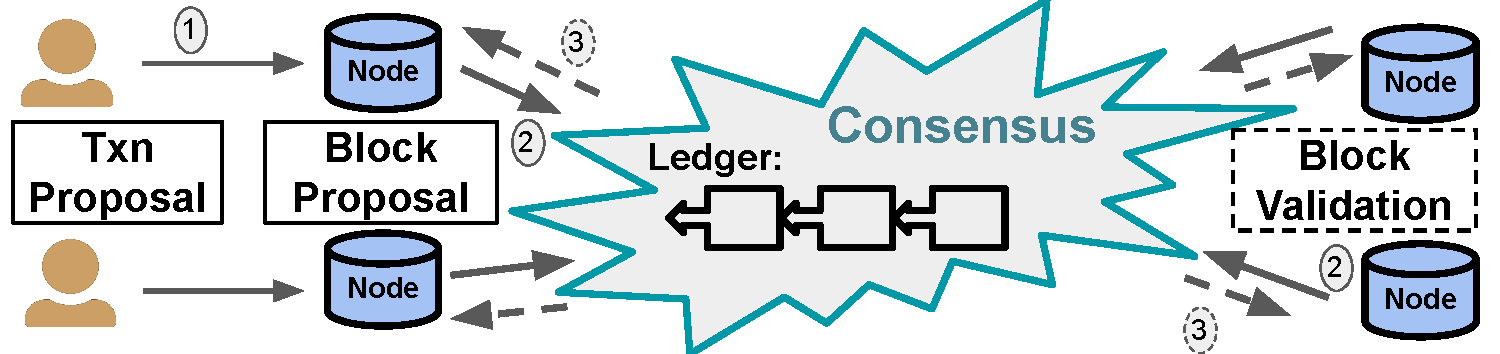
\includegraphics[width=0.99\textwidth]{diagram/literature/ox_arch.pdf}
    \end{subfigure}
    \begin{subfigure}{0.8\textwidth}
      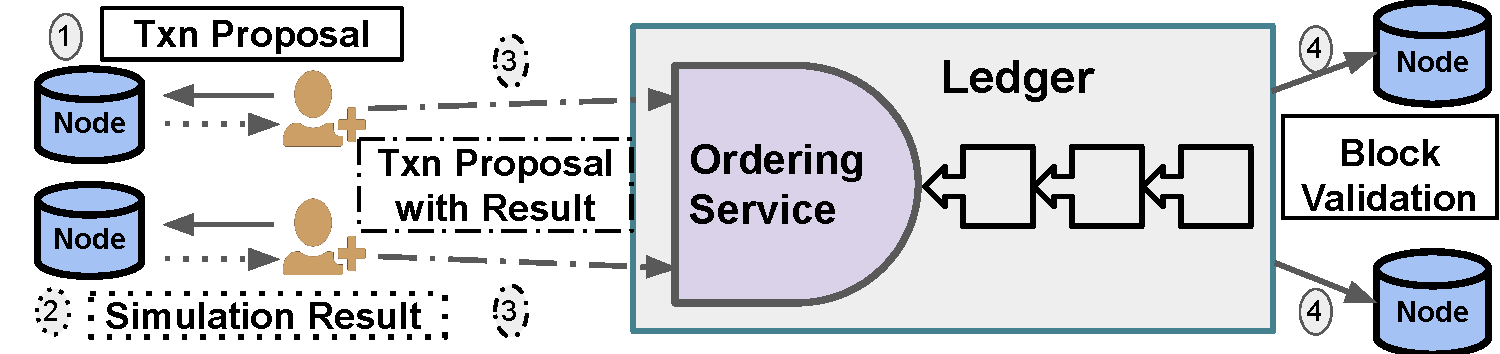
\includegraphics[width=0.99\textwidth]{diagram/literature/eov_arch.pdf}
    \end{subfigure}
    \caption{Order-execute vs. Execute-order-validate architecture. }
    \label{diagram:literature:execution}
    % \vspace{-1.0em}
\end{figure}

\subsection{Order-execute Architecture}
In the Order-execute architecture, each peer serially executes transactions, based on the established order according to the ledger by the consensus. 
Bitcoin as well as all cryptocurrency-based blockchain adopts this concurrency-free design, simply because the consensus, rather than the execution layer, decides on the system performance. 
Moreover, sequentiality makes it easy to reason about the system behavior. 

Despite this, things still get convoluted when transactions deal with Turing-complete logic. For example, many security researchers have demonstrated that Solidity contracts in Ethereum are far more tricky than expected~\cite{luu2016making,parizi2018smart,atzei2017survey}. 
Due to some subtle misunderstanding on operation semantics on EVM, flawed contracts can be exploited by adversaries to gain profits. 
And the problem is further exaggerated given the transparency and the irreversibility of blockchains. 
The DAO hack shows that such an attack is not only a possibility in the theory but a true threat in reality~\cite{santos2018dao}.
In the meantime, there come along a series of empirical guidelines and practical tools to aid the contract development~\cite{ducasse2019open,jeng2019step,bai2018formal,tikhomirov2018smartcheck}. 

Through the Order-execute architecture takes on the sequential approach, it is never insulated from the concurrency topic. 
For example, after remarking the reminiscence between contract bugs in blockchains and data races in shared-memory programming, researchers propose a novel viewpoint on the security issues of contracts, from the concurrency perspective in distributed computing~\cite{herlihy2019blockchains,sergey2017concurrent}. 
In ~\cite{dickerson2019adding}, researchers explore to tentatively execute transactions in parallel and then fall into serial if encountering a conflict.  
Instead of speeding up the entire system, the goal of the concurrency is to facilitate the block validation, so that validators can gain a competitive edge on the next block mining. 
Quantitative analysis of the transaction graph shows abundant concurrent chances in mainstream blockchains~\cite{reijsbergen2020exploiting,saraph2019empirical}. 

\subsection{Execute-order-validate Architecture}
Execute-order-validate architecture is proposed in Hyperledger Fabric v1.0~\cite{androulaki2018hyperledger}. 
Rather than taking a monolithic approach, the system is designed with two types of blockchain nodes: peers which execute smart contracts and validate blocks, and orderers which order transactions. 
A transaction pipeline is divided into three phases. 
In the Execute phase, a client requests a subset of peers to execute the transaction speculatively. 
The client collects the results and signatures from peers and sends them to the orderers. 
In the Order phase, orderers order the transactions and batch them into blocks.
For modularity, orderers do not inspect the transaction details. 
In the Validate phase, each peer pulls blocks from the orderers and independently validates each block before persisting the results. 
The block validation process firstly verifies whether transactions satisfy the endorsement policy, i.e., enough number of peers show the endorsement by their signature. 
Then validation procedure checks for conflicts in the read/write sets for each transaction. 
The invalid transactions will not persist their effects, even though they are part of the ledger. 
Read-only queries only involve the Execute phase. 

This architecture brings additional benefits compared to Order-execute architecture. 
Firstly, the endorsement policy decouples the trust condition of a contract from the consensus. 
For example, a valid transaction may carry the execution results from only one of three peers. 
In contrast, the Order-execute architecture mandates the majority of peers to agree on the contract result. 
Secondly, it preserves confidentiality by restricting the execution to specify peers.
Clients, aware of the results before transactions are effected, can also minimize the uncertainty. 
Lastly, speculative execution at the start fits well for the concurrency.
It greatly facilitates computation-heavy transactions, which would queue up in Order-execute architecture. 

However, such concurrency comes with the cost, which manifests as the aborted transactions for the serializability. 
We have empirically demonstrated that in Figure~\ref{chart:intro:basic} and will elaborate this issue in Chapter~\ref{ch:txn}. 
In light of this, Fabric++ reorders transactions during the Order phase to minimize the abort~\cite{sharma2019blurring}. 
OXII architecture is featured for an additional dependency resolution phase at the start~\cite{amiri2019parblockchain}.
So that it enables for a concurrency-friendly transaction schedule. 
OXII relies on the core assumption that the dependency can be extracted by inspecting the contract codebase. 
In the same spirit, XOX architecture runs a patch-up code to streamline a contended transaction~\cite{gorenflo2020xox}. 
The dependency captured during the transaction execution determines this snippet of code. 

\section{Consensus Layer}
Byzantine-tolerant consensus differentiates blockchains from other distributed systems. 
Proof-of-work (PoW), initially proposed in Bitcoin, opens up a new horizon on incentive-based protocols. 
Meanwhile, the permissioned blockchains revitalize the interest of 
state machine replication approach to address the arbitrary failure. 

\subsection{PoW and its Analysis}
The essence of PoW is a hard-to-solve and easy-to-verify puzzle. 
The protocol prescribes that the first solver has the privilege to broadcast a new block on the tip of the ledger. 
By adjusting the puzzle difficulty such that the solving duration exceeds the maximum network delay,
all blockchain participants can then sync up on the unique chain. 
In Bitcoin, the puzzle solution is a nonce to make the block hash value prefixed with enough zeros. 
The block proposer gets compensated for the hashing power with the newly-minted cryptocurrencies and the transaction fee. 

In the context of Bitcoin, the solution-finding process is called \textit{mining}. 
Due to the irreversibility of the hash function, mining is fair to all participants, including the adversaries. 
Ruling out the possibility that adversaries control the majority of the hash power, it results into the following two implications.
If the adversaries pour all their resources to mine on a shorter chain fork, 
that fork can catch up the longest chain with negligible probability, where the rest of honest power concentrates. 
Nakamoto has bounded this possibility to be exponentially small in the original whitepaper~\cite{nakamoto2019bitcoin}.
More in-depth mathematical frameworks have been established to reason the mining behavior ~\cite{gervais2016security,kiayias2015speed,ren2019analysis,miller2014anonymous,garay2015bitcoin}. 
On the other hand, honest block proposers, aware that the longest chain is hardly revertible, are incentivized to extend on it. 
It is because their proposed block contains a coinbase transaction that credits proposers to the minted cryptocurrencies. 
Only the block is in the longest chain then this transaction can take into effect. 

Inevitably, the longest-chain-rule may lead to two divergent forks during the asynchronous network period. 
When the network delay exceeds the block interval, two honest participants may generate two different blocks but on the same height. 
The longest-chain-rule will eventually resolve to a unique chain when the network partition heals.
Hence, transactions in the ledger may not be secure given that they might reside on a shorter, to-be-pruned fork. 
Considering this, clients are advised to wait for their transactions until deep enough, before considering them committed. 
Intuitively, this depth, quantified by the number of blocks behind, balances between latency and security. 
In the meantime, the block interval and the block size controls the tradeoff between throughput and security. 
The shorter interval and the larger block imply greater system capacity. 
But it compromises the security, i.e., the network may not propagate a block to each participant before the next block is generated. 

Moreover, \cite{eyal2014majority} suggests that adversaries may not be incentivized to follow the default mining policy, i.e., mining on the longest chain and broadcast the block immediately. 
Instead, they may temporally withhold mined blocks and selectively publish them to gain extra profits.
Since then, more mining policies are discovered which allows adversaries to gain a competitive edge \cite{nayak2016stubborn,courtois2014subversive},
even infiltrating other mining pools to waste their resources~\cite{luu2015power,eyal2015miner}. 
Researchers employ a Markov Decision Process to find the optimal mining policy and explore the performance-security tradeoff~\cite{gervais2016security,sapirshtein2016optimal}.

\subsection{The Enhancements on PoW}
PoW has long been plagued for its energy assumption. 
In 2019, Bitcoin's electricity consumption is reported to reach 45.8 TWh. 
Naturally, several researchers propose to transform PoW to be more eco-friendly, 
or at least dedicate resources to useful tasks. 
We refer to these PoW-based enhancements as Proof-of-X (PoX). 

The major challenge of PoX is to replace the original computation-intensive puzzle and preserve its long-to-solve and easy-to-verify nature. 
For example, Proof-of-Stake (PoS) requires miners to stake a certain amount of cryptocurrencies~\cite{king2012ppcoin}. 
The stake will be confiscated if the proposed blocks are found to be invalid. 
One can find the adoption of PoS in the following blockchains~\cite{kiayias2017ouroboros,david2018ouroboros,bentov2016snow} and their security analysis in~\cite{nguyen2019proof,li2017securing,brown2019formal}. 
Proof-of-Elapsed-Time (PoET) replies on the Trusted Execution Environment to attest block validators that miners have waited enough time before the next block proposal~\cite{chen2017security}. 
To fully exploit the consumed resources to useful works, 
Proof-of-Retrievability is repurposed for the data archival~\cite{miller2014permacoin}, Proof-of-Prime-Number for the prime number searching~\cite{king2013primecoin}, and others for matrix product problems~\cite{shoker2017sustainable}. 

Another enhancement direction is to optimize the primitive PoW. 
Researchers adapt the puzzle-computation to resist ASIC-equipped mining and deter power centralization~\cite{zamanov2018asic,cho2018asic}. 
On the other hand, they refine the PoW mechanism to increase the system capacity.
For example, the original PoW groups the leader election and transaction proposal together. 
Bitcoin-NG decouples these two tasks, by allowing a puzzle solver to continuously propose transactions until the next solver emerges~\cite{eyal2016bitcoin}. 
GHOST incentives miners to extend on the heaviest sub-tree instead of the longest chain~\cite{sompolinsky2015secure}. 
This is to better recycle orphaned blocks. 
Conflux furthers replies on GHOST to determine the pivot chain and use the pivot chain to decide on a direct-acyclic graph, whose topological order determines the overall transaction sequence~\cite{li2018scaling}. 
The OHIE is renowned for its multiple-chain structure to harness the distributed network setup~\cite{yu2020ohie}. 
Its protocol drives each chain to catch up at the same height. 

\subsection{Byzantine Fault-tolerant Consensus}
The state-machine replication method to address byzantine consensus resurges with the popularity of blockchains. 
The Byzantine-fault tolerant consensus problem involves a number of nodes with initial divergent proposals. 
The problem requires honest nodes to reach agreement on one of the proposals, while reserving the safety (no possibility of disagreement) and liveness (guarantee of termination)~\cite{lamport2019byzantine}. 
And this must hold true under the premise that a fraction of malicious nodes may perform arbitrary action. 
Compared to Bitcoin, this problem modeling is more general, i.e., it is not targeting only on the ledger and no incentives can be hinged on. 

Long before Bitcoin, PBFT has provided the first-ever practical approach.
It achieves the consensus in $O(n^2)$ message complexity where $n$ is the number of nodes. 
Quorum adopts a PBFT-variant, IBFT as one of its consensus options but still requires for $O(n^2)$ messages~\cite{saltini2019correctness}. 
Tendermint reduces this bound to $O(n)$ but forgoes the network responsiveness~\cite{buchman2016tendermint}. 
In a word, unlike PBFT, the progress of Tendermint is dependent on the maximum network delay, rather than the actual message transmission delay~\cite{amoussou2019dissecting}. 
Hotstuff augments on the two-phase approach of PBFT and Tendermint into three phases of the message exchange~\cite{yin2019hotstuff}. 
But it achieves both network linearity ($O(n)$ message complexity) and the responsiveness. 

While the above series of researches are rooted from PBFT, researchers in VMWare address the problem from a new angle. 
They remark the possibility to reach consensus in a single phase, given more number of nodes have acknowledged the proposal than normal. 
Based on this insight, they starts from Fast Byzantine Paxos~\cite{martin2006fast} and Zyzzyva~\cite{gueta2019sbft}, and leads into a series of re-analysis~\cite{abraham2017revisiting} and re-design~\cite{abraham2018revisiting, gueta2019sbft}. 
Their novelty comes from a fast path if more-than-normal acknowlegements have been collected before a timeout. 
Otherwise, the consensus falls backs to the standard two-phase pipeline.  

FLP Impossibility Result imposes no deterministic, safe and live protocols under the asynchronous network~\cite{fischer1985impossibility}. 
The above protocols trade the liveness for the safety during the network partition. 
In other words, disagreement never occurs even the network loses the connection. 
Correspondingly, there also exist a number of approaches that rely on the network synchrony for the safety~\cite{abraham2020sync,abraham2017efficient}. 
In this manner, these protocols behave like PoW in Bitcoin, i.e., a chain will fork under the asynchronous period. 
In their design, the strict network assumption comes into play when to reliably broadcast the latest, majority-acknowledged block proposal. 
Notably, Flexible BFT mixes two types of deterministic protocols together, so that clients can draw their own commit decisions at their discretion on the network condition~\cite{malkhi2019flexible}. 

Randomness is another alternative route to break the Impossibilty, in order to reach agreement on the ledger. 
For example, HonestBadgerBFT combines a variety of randomized agreement protocols~\cite{miller2016honey}. 
So that it achieves linear message complexity, as PoW in Bitcoin. 
As the carry-on work, BEAT provides a diversity of randomized protocols that tailors for various application demands~\cite{duan2018beat}. 
Such randomization takes in the form of the unpredictable network connectivity in~\cite{rocket2019scalable}.
In its design, each node repetitively queries for the proposals the neighbors that it knows of. 
It then determines his own proposal from the majority of query results and uses it to respond for other's queries. 
Eventually, all honest nodes are probabilistically steered towards a uniform outcome, even though a limited fraction may cheat. 

\subsection{Committee-based Consensus}
Blockchains with the committee-based consensus select a single or multiple representative committees, which then establish the ledger with the above state-machine replication consensus. 
This idea has been dated back to PeerCensus~\cite{decker2016bitcoin}. 
But their application may not be that straightforward. 
It is because these off-the-shelf protocols require for strong assumptions, including identity management, member constitution, and so on. 
To cater for these conditions, most blockchains must couple wth some additional procedures, especially on the fair committee formation. 
For example, Algorand determines a single committee based on the Verifiable Random Function (VRF)~\cite{gilad2017algorand}. 
In particular, nodes must compute a value with VRF from its private key and a common seed. 
Only those with specific values are allowed to join the consensus with their public keys. 
VRF remains unpredictable without knowing the common seed beforehand. 
By starting from an unbiased random seed, Algorand guarantees that no adversaries may dominate a committee. 
Omniledger depends on the Randhound to achieve the decentralized and unbiased randomness, and power the multi-committee establishment~\cite{kokoris2018omniledger}. 
Byzcoin repurposes PoW to determine the membership for a single committee~\cite{kogias2016enhancing}. 
PoW not only guarantees the randomness but also resists the Sybil attacks under the permissionless setting. 
RapidChain also uses PoW to determine participants, from which it breaks into multiple committees with a theoretical-involved method~\cite{zamani2018rapidchain}. 
Elastico directly uses PoW nonce and group solvers with common prefixes into one of the committees~\cite{luu2016secure}. 
Such randomness for the committee formation comes from Trusted Execution Environment in AHL~\cite{dang2019towards}.
Not that all the above systems are subject to the periodic committee re-configuration between epochs. 
This prevents adaptive adversaries to exploit the setup and infiltrate honest nodes. 
The reconfiguration can be a full swap like in Elastico~\cite{luu2016secure}, Algorand~\cite{gilad2017algorand}, and Omniledger~\cite{kokoris2018omniledger}, or in a rotational manner like Byzcoin~\cite{kogias2016enhancing}, RapidChain~\cite{zamani2018rapidchain}, and AHL~\cite{dang2019towards}. 

We also observe several blockchains adopt a non-technical solution on membership management. 
For instance, a central authority decides on the validators' role in RSCoin~\cite{danezis2015centrally}. 
The participants and their weight in Libra~\cite{baudet2019state} and EoS~\cite{xu2018eos} are pre-determined according to their initial investment. 
Chainspace completely sidesteps the committee formation problem~\cite{al2017chainspace}. 
It leaves the behavior of malicious committee audible under the premise that they can be enforced by an external entity.

\section{Application}
Blockchains provide unique decentralization, auditability, transparency, and irreversibility, adding abundant value to real-world applications. 
The most natural use case is to rely on the decentralized ledger as a trustworthy chronological logbook. 
For example, the Bitcoin protocol allows for a 40 byte of arbitrary data piggybacked at \textit{OP\_RETURN} opcode~\cite{opreturn}.
Several applications exploit this payload to use as a message commitment. 
So that one in the future can verify its existence, the creation time and the source of the origin. 
More advanced usage can be found in~\cite{maesa2017blockchain}, where this payload is used to encode the right transfer of the external resource access, and in~\cite{wu2017voting} for the e-voting. 
This survey investigates a broader range of applications and quantifies their the overhead of the piggybacking scheme~\cite{bartoletti2017analysis}. 

Another popular application is the token management.
Unlike the built-in cryptocurrency, the token is associated with external assets. 
The assets may range from vouchers, IOU, copyrights, and tangible objects. 
So that one may redeem the asset in the world, by showing the cryptographic proof on the token possession in the blockchain. 
For example, one may get a one-for-one exchange between Tether tokens and US dollars. 
We observe most of these applications operate on Ethereum, especially to hinge on the official provided ERC20 token standard~\cite{wiki:ERC20}.
In particular, ERC20 is a smart contract that defines a common list of rules on token operations.  
Any token issuer can deploy its own version of the ERC20 contract with the prevision of the initial ownership and the total of the supply amount. 
The transfer of tokens takes in the form of the contract invocations. 
So that their transactions are secured by Ethereum.
ERC20 token is widespread with a growing number of Initial Coin Offering (ICO). 
This study reveals that there are more than 64k distinct ERC20 tokens~\cite{victor2019measuring}.
We refer readers to~\cite{victor2019measuring,somin2018network,chen2020traveling} for the analysis of their transaction pattern. 

To further unleash the blockchain potential, plenty of business proposals explore its intermediary-free data processing capabilities to the banking industry~\cite{guo2016blockchain}, the supply chain management~\cite{tse2017blockchain,saberi2019blockchain,korpela2017digital}, Internet-of-Things(IoT)~\cite{novo2018blockchain,huh2017managing,khan2018iot}, the autonomous governance~\cite{diallo2018egov,atzori2015blockchain}, identity service~\cite{lim2018blockchain,lootsma2017fintech}, medical record ownership control~\cite{azaria2016medrec,medilot}, collaborative shared databases~\cite{peng2020falcondb,el2019blockchaindb} and so on. 
In all the above cases, blockchains provide a unique trust-building platform that coordinates the business process.
The procedure usually involve multiple stakeholders with the conflict of interest. 
Along with the popularity, some researchers voice out their concern about the improper blockchain usage. 
\cite{wust2018you} criticizes this worrying trend by critically analyzing several unreasonable cases. 
\cite{yaga2019blockchain,chowdhury2018blockchain,wust2018you} provide empirical guidelines for applications to choose between blockchains and conventional databases. 
In their opinion, the absence of the central authority is the deciding factor for the blockchain adoption. 
This absence may be due to the entangled interest in the application, the trust deficit from the hostile environment or etc. 
Otherwise, the expense of dis-intermediation, in terms of the extra storage and performance, far outweighs other blockchain-provided features. 
Most similar business requirements, such as the provenance support and state integrity, can be more efficiently satisfied with other technical solutions.
For example, QLDB, as a centrally administrated, in-cloud database, provides a verifiable storage~\cite{qldb}. 
In other words, the QLDB vendor is technically possible to tamper the data or refuse to deliver the service, despite the fact that all this action will leave evidence. 
Blockchains, however, is capable to prevent such arbitrary behavior due to their decentralized consensus. 
But it is questionable whether such additional security guarantee is worthwhile for most applications. 

\section{Benchmarks and Surveys}
Even though the aforementioned references cover most representative research works, they are far from comprehensive to draw an overall picture on the recent blochchain progress. 
For a wider range of exposition, we compile blockchain-related surveys with respect to their focused layers in Table~\ref{tab:literature:survey}. We also tabulate reported benchmarks with their selected systems in the table.

\begin{table}[]
  \caption{Blockchain-related surveys and benchmarks}
  \label{tab:literature:survey}
  \centering

  \begin{tabular}{l|l|l}
    \hline
                             & \textbf{Layer} & \textbf{Focus}                                                                                       \\ \cline{2-3} 
    \multirow{4}{*}{\textbf{Surveys}} & Execution      & Ethereum Contract Security~\cite{li2020survey,atzei2017survey,chen2020survey,praitheeshan2019security}                                                                           \\ \cline{2-3} 
                             & Consensus     &  \cite{wang2019survey,nguyen2018survey,xiao2020survey,garay2020sok}                                                                                                 \\ \cline{2-3} 
                             & Application    & \begin{tabular}[c]{@{}l@{}}Internet-of-Things~\cite{novo2018blockchain,wu2019comprehensive,wang2019iotsurvey} \\ Banking~\cite{guo2016blockchain,cocco2017banking,peters2016understanding} \\ Others~\cite{mollah2020blockchain,al2019blockchain,blossey2019blockchain,zhuang2020blockchain}\end{tabular}                                  \\ \cline{2-3} 
                             & Others         & \begin{tabular}[c]{@{}l@{}}Technical Overview~\cite{zheng2018blockchain,lin2017survey,dinh2018untangling}\\ Chain Interoperability and Sharding~\cite{zamyatin2019sok,wang2019sok,yu2020survey}\\ Data Privacy~\cite{feng2019survey,joshi2018survey,mohanta2019blockchain} \end{tabular} \\ \hline
    \multicolumn{2}{l|}{\textbf{Benchmarks}}           & \begin{tabular}[c]{@{}l@{}}Hyperledger Fabric~\cite{dinh2017blockbench,thakkar2018performance,nasir2018performance,ruan2019blockchains,pongnumkul2017performance,tinguely2019benchmarking}\\ Ethereum\cite{dinh2017blockbench,pongnumkul2017performance,rouhani2017performance,chen2018comparative} \\ Quorum~\cite{ruan2019blockchains,baliga2018performance} \\ Parity~\cite{dinh2017blockbench} \\ Corda~\cite{cordaperf,tinguely2019benchmarking} \end{tabular}                                  \\ \hline
    \end{tabular}
\end{table}

\section{Lessons learnt from the Review} 
Our above review reveals a mismatch between the focus of the industry and academia on blockchains. 
In particular, researchers place great emphasis on their security aspects. They restrict their attention on the incentive-based consensus, and UTXO-based cryptocurrency in permissionless blockchains. On the other hand, entrepreneurs in the industry show the most interest in the intermediary-free data processing capabilities from permissioned blockchains. 
In the meantime, we observe most researchers treat a blockchain as it is, but few of them realize its vast similarities to distributed databases. A few work with this awareness juxtapose permissioned blockchains and distributed databases for the joint study. 
But their analysis leaves much room for improvement: they either only show the blockchains' inferior performance to databases~\cite{dinh2017blockbench,chen2018comparative}. Or they compare their distinct value-addition properties for applications~\cite{chowdhury2018blockchain,wust2018you,yaga2019blockchain}. 
But they ignore a promising area, which is to optimize permissioned blockchains with database-specific techniques to support general workloads. 

Our thesis moves a step forward along this direction. 
We first classify blockchains and distributed databases under the same taxonomy.
Based on this framework, we jointly understand their design choices and behavior (Chapter \ref{ch:twin}). 
With the developed insights, we extend the provenance support to smart contracts to improve utility (Chapter \ref{ch:prov}). Then learning from databases, we explore reordering techniques to reduce the transaction abort. 
This performance enhancement applies to any blockchains with execute-order-validate execution pipeline (Chapter \ref{ch:txn}).  

